\documentclass[12pt]{article}

% UTF-8 encoding and fonts
\usepackage[utf8]{inputenc}
\usepackage[T1]{fontenc}
\usepackage{lmodern}

% Page setup
\usepackage[margin=1in]{geometry}
\usepackage{setspace}
\onehalfspacing

% Typography
\usepackage{microtype}

% Math and symbols
\usepackage{amsmath,amssymb}

% Graphics
\usepackage{graphicx}
\usepackage{float}
\usepackage{subcaption}

% Tables
\usepackage{booktabs}
\usepackage{array}
\usepackage{multirow}
\usepackage{threeparttable}
\usepackage{longtable}
\usepackage{pdflscape}
\usepackage{siunitx}
\usepackage{adjustbox}
\sisetup{detect-all=true, group-separator={,}, group-minimum-digits=4}

% Bibliography
\usepackage{natbib}
\bibliographystyle{aer}

% Hyperlinks
\usepackage{hyperref}
\hypersetup{
    colorlinks=true,
    linkcolor=blue,
    citecolor=blue,
    urlcolor=blue
}
\usepackage[nameinlink,noabbrev]{cleveref}

% Timing data
\IfFileExists{timing_data.tex}{\input{timing_data.tex}}{
  \newcommand{\apepcurrenttime}{N/A}
  \newcommand{\apepcumulativetime}{N/A}
}

% Captions
\usepackage{caption}
\captionsetup{font=small,labelfont=bf}

% Section formatting
\usepackage{titlesec}
\titleformat{\section}{\large\bfseries}{\thesection.}{0.5em}{}
\titleformat{\subsection}{\normalsize\bfseries}{\thesubsection}{0.5em}{}

% Custom commands
\newcommand{\E}{\mathbb{E}}
\newcommand{\Var}{\text{Var}}
\newcommand{\Cov}{\text{Cov}}
\newcommand{\ind}{\mathbb{I}}
\newcommand{\sym}[1]{\ifmmode^{#1}\else\(^{#1}\)\fi}

\title{Do Red Flag Laws Reduce Violent Crime? Evidence from Staggered State Adoption}
\author{APEP Autonomous Research\thanks{Autonomous Policy Evaluation Project. Correspondence: scl@econ.uzh.ch} \and @olafdrw}
\date{\today}

\begin{document}

\maketitle

\begin{abstract}
\noindent
Between 1999 and 2020, nineteen U.S. states adopted Extreme Risk Protection Order (ERPO) laws---commonly called ``red flag'' laws---allowing courts to temporarily remove firearms from individuals deemed dangerous. I exploit this staggered adoption using the \citet{callaway2021difference} heterogeneity-robust difference-in-differences estimator with FBI Uniform Crime Reports data covering all 50 states from 2000 to 2023. The preferred specification yields a murder rate ATT of $-0.251$ per 100,000 (SE $= 0.224$), a directionally negative but statistically insignificant reduction. Standard two-way fixed effects overestimates this effect by 3.6 times ($-0.916$, $p < 0.01$), demonstrating substantial heterogeneity bias. Results are robust across seven alternative specifications, with leave-one-out ATTs confined to $[-0.380, -0.187]$. The analysis finds suggestive evidence of modest crime-reducing effects concentrated among states permitting family-member petitions, though statistical power limits definitive conclusions.
\end{abstract}

\vspace{1em}
\noindent\textbf{JEL Codes:} K14, K42, H75 \\
\noindent\textbf{Keywords:} red flag laws, ERPO, violent crime, gun policy, difference-in-differences, staggered adoption

\newpage

\section{Introduction}

In February 2018, a 19-year-old former student killed 17 people at Marjory Stoneman Douglas High School in Parkland, Florida. Within three weeks, Florida enacted an Extreme Risk Protection Order (ERPO) law---one of seven states to adopt such legislation that year. By 2024, twenty-one states had passed some form of red flag law (nineteen by the end of 2020, with two more in 2024), making ERPOs the fastest-growing category of firearm regulation in the United States. Yet whether these laws actually reduce violent crime remains an open question: the RAND Corporation's comprehensive review rates the evidence as ``inconclusive'' \citep{smart2023rand}.

This paper provides the first multi-state causal analysis of ERPO laws' effects on violent crime using modern heterogeneity-robust methods. The existing literature suffers from two limitations. First, most credible causal studies examine single states---Connecticut \citep{swanson2020erpo}, Indiana \citep{kivisto2015effects}, California \citep{pear2022gvro}, or Florida \citep{florida_erpo2024}---making generalization difficult. Second, the handful of multi-state analyses rely on standard two-way fixed effects (TWFE), which \citet{goodman2021difference} and \citet{dechaisemartin2020two} show can produce severely biased estimates under treatment effect heterogeneity---precisely the setting here, where states adopted at different times and with varying law designs.

I exploit the staggered adoption of ERPO laws across 19 states between 1999 and 2020 using the \citet{callaway2021difference} doubly-robust difference-in-differences estimator with FBI Uniform Crime Reports (UCR) data \citep{kaplan2021ucr}. The identification strategy leverages the fact that states adopted ERPO laws at different times, with 31 never-adopting or not-yet-treated states serving as the primary control group. The Callaway-Sant'Anna estimator avoids the negative weighting problems that plague TWFE by separately estimating group-time average treatment effects for each adoption cohort, then aggregating them into an overall treatment effect.

The main finding is a point estimate suggesting modest crime-reducing effects that do not reach conventional significance levels. The preferred specification yields an overall ATT on the murder rate of $-0.251$ per 100,000 population (SE $= 0.224$, $p = 0.262$), corresponding to a 4.9\% reduction relative to the pre-treatment mean. For comparison, standard TWFE estimates a highly significant effect of $-0.916$ ($p < 0.01$), overstating the magnitude by a factor of 3.6. This divergence is itself an important methodological finding: it demonstrates that existing TWFE-based evidence on ERPO effectiveness is unreliable.

The results are stable across seven robustness specifications. Using not-yet-treated controls ($-0.212$), dropping the 2021 UCR transition year ($-0.201$), restricting to the pre-COVID period ($-0.054$), and dropping the large 2018 adoption cohort ($-0.129$) all produce directionally consistent estimates. The leave-one-state-out exercise shows ATTs bounded between $-0.380$ and $-0.187$, confirming that no single state drives the results. Randomization inference yields a two-sided $p$-value of 0.469, consistent with the asymptotic inference. The log specification suggests a $-5.3\%$ effect on murder rates (SE $= 3.98\%$), close to the lower bound of prior single-state estimates.

Heterogeneity analysis by law design reveals that states permitting family members to petition for ERPOs (in addition to law enforcement) show larger point estimates ($-0.311$) than states restricting petitions to law enforcement only ($-0.057$). This pattern is consistent with the hypothesis that family members possess private information about escalating risk that law enforcement lacks \citep{wintemute2019extreme, webster2020erpo}. However, neither estimate achieves significance, and the small number of law-enforcement-only states (Indiana and Florida in the CS-DiD sample) limits inference.

This paper contributes to three literatures. First, it advances the empirical evaluation of ERPO laws beyond single-state case studies by providing the first multi-state analysis using heterogeneity-robust DiD methods. While the suicide-reduction channel is well established \citep{kivisto2015effects, deangelis2023red}, the violent crime channel has received far less rigorous scrutiny. Second, it contributes to the methodological debate on TWFE bias in applied policy evaluation \citep{goodman2021difference, roth2023pretest, borusyak2024revisiting} by documenting a 3.6-fold overestimation in a high-stakes policy setting. Third, it informs the active policy debate over ERPO adoption: as of 2024, six states have enacted ``anti-ERPO'' laws prohibiting such orders, and the gap between political rhetoric and empirical evidence is large \citep{luca2020impact}.


\section{Institutional Background}

\subsection{What Are ERPO Laws?}

Extreme Risk Protection Orders---also known as ``red flag'' laws, gun violence restraining orders (GVROs), or risk warrants---are civil court orders that temporarily prohibit individuals from purchasing or possessing firearms when they are deemed to pose a danger to themselves or others. Unlike criminal proceedings, ERPOs are preventive: they operate before violence occurs, based on demonstrated risk rather than past offenses.

The typical ERPO process involves three stages. First, an eligible petitioner (law enforcement officer, family member, or in some states, medical professionals or educators) files a petition in state court alleging that an individual poses a significant danger of causing personal injury. Second, a judge evaluates the evidence and may issue a temporary ex parte order, typically lasting 14--21 days, requiring the respondent to surrender firearms. Third, a full hearing is held where the respondent can contest the order, and the judge decides whether to issue a final ERPO, typically lasting 6--12 months with the possibility of renewal.

\subsection{Staggered Adoption Across States}

Connecticut became the first state to enact an ERPO law in 1999, followed by Indiana in 2005. Adoption remained limited until 2016, when California and Washington passed laws, creating the first cohort of the modern adoption wave. The pivotal year was 2018, when mass shootings---particularly the Parkland massacre in February---catalyzed rapid legislative action. Seven states adopted ERPOs in 2018: Florida, Vermont, Rhode Island, Massachusetts, Maryland, Delaware, and Oregon. Four more states followed in 2019 (Colorado, New Jersey, New York, Illinois) and four in 2020 (Hawaii, Nevada, New Mexico, Virginia). Minnesota and Michigan subsequently adopted ERPOs in 2024, after the sample period ends; they are treated as not-yet-treated in the analysis.

This staggered adoption pattern is critical for identification. The variation in timing means that states entering treatment at different times can serve as controls for one another. The 2018 wave, comprising seven states, is the largest adoption cohort and provides a natural focus for many specifications.

\subsection{Heterogeneity in Law Design}

A key dimension of variation across ERPO laws is who may petition. In ``law enforcement only'' (LE-only) states---Connecticut, Indiana, and Florida---only police officers or prosecutors can file for an ERPO. In ``family petition'' states, family members, household members, and sometimes medical professionals or school officials can also petition. This distinction matters because it determines the pool of private information available to the system: family members may observe warning signs---escalating threats, substance abuse, mental health crises---that never reach law enforcement attention \citep{wintemute2019extreme}.

The duration, standard of proof, and penalties for violation also vary. Most states require ``preponderance of the evidence'' for temporary orders and ``clear and convincing evidence'' for final orders. These differences are important for understanding heterogeneous treatment effects but are difficult to exploit empirically due to correlation with adoption timing.

\subsection{The Counter-Movement: Anti-ERPO Legislation}

Not all states have moved toward ERPOs. Six states---Oklahoma, Tennessee, West Virginia, Wyoming, Montana, and Texas---have enacted legislation explicitly prohibiting or restricting ERPO-type orders. These ``anti-ERPO'' laws serve as a useful placebo group, as they represent a deliberate policy choice against firearm removal mechanisms.

\subsection{Mechanisms: How Might ERPOs Reduce Crime?}

The primary mechanism through which ERPOs could reduce violent crime is straightforward: temporary firearm removal from high-risk individuals prevents firearm-facilitated violence. This operates through at least three channels:

First, \textit{direct prevention}: by removing firearms from individuals in crisis, ERPOs mechanically prevent firearm homicides and assaults that would otherwise have occurred. \citet{cook1979effect} established that weapon availability affects the lethality of violent encounters, and the substitution to less-lethal weapons is imperfect.

Second, \textit{deterrence}: the existence of ERPO laws may deter individuals from making threats or engaging in escalating behavior, knowing that such behavior could trigger firearm confiscation.

Third, \textit{intervention catalyst}: the ERPO process often brings respondents into contact with mental health services, substance abuse treatment, or domestic violence intervention programs, potentially addressing underlying risk factors.

The established channel for ERPO effectiveness is suicide prevention: \citet{kivisto2015effects} found significant reductions in firearm suicides in Connecticut and Indiana, and \citet{deangelis2023red} confirmed this with nationwide data. The violent crime channel is less well-established, partly because ERPO usage for interpersonal violence risk (as opposed to self-harm risk) varies substantially across jurisdictions.


\section{Data}

\subsection{FBI Uniform Crime Reports}

The primary outcome data come from the FBI Uniform Crime Reporting (UCR) program, accessed through the Kaplan Concatenated Files hosted at Harvard Dataverse \citep{kaplan2021ucr}. The UCR Offenses Known and Clearances by Arrest dataset provides agency-level counts of crimes reported to and recorded by law enforcement agencies across the United States.

I aggregate agency-level data to the state-year level, restricting to agencies that reported for all 12 months in a given year to ensure consistent coverage. The key outcome variables are: murder and non-negligent manslaughter, aggravated assault, robbery, and the composite measures of violent crime (murder $+$ rape $+$ robbery $+$ aggravated assault) and property crime (burglary $+$ larceny-theft $+$ motor vehicle theft). All outcomes are expressed as rates per 100,000 population.

The analysis sample spans 2000--2023 and covers all 50 states (excluding the District of Columbia and territories). This yields a balanced panel of 1,200 state-year observations.

\subsubsection{Data Limitations}

The UCR data have well-known limitations. First, participation is voluntary, and reporting completeness varies across agencies and years. The restriction to 12-month reporters mitigates this but may introduce selection if non-reporting agencies differ systematically. Second, 2021 represents a transition year when the FBI shifted from the Summary Reporting System (SRS) to the National Incident-Based Reporting System (NIBRS), leading to reduced coverage. I flag 2021 observations and test robustness to their exclusion.

\subsection{ERPO Treatment Coding}

I compile ERPO adoption dates from the National ERPO Resource Center (erpo.org) and cross-validated against three independent sources: the Giffords Law Center, Everytown for Gun Safety, and Ballotpedia. The treatment variable is defined as a binary indicator equal to one for state $s$ in year $t$ if an ERPO law was in effect for the majority of that calendar year.

Table~\ref{tab:erpo_states} presents the 19 states that adopted ERPOs within the sample window, with their adoption years and petitioner types. Note that Connecticut (adopted 1999) is treated before the panel begins in 2000 and is therefore automatically excluded from CS-DiD estimation, leaving 18 effectively treated states.

\begin{table}[H]
\centering
\caption{ERPO Law Adoption by State}
\label{tab:erpo_states}
\begin{adjustbox}{max width=\textwidth}
\begin{tabular}{llcl}
\toprule
State & Abbreviation & Year Enacted & Petitioner Type \\
\midrule
Connecticut & CT & 1999 & LE only \\
Indiana & IN & 2005 & LE only \\
California & CA & 2016 & Family + LE \\
Washington & WA & 2016 & Family + LE \\
Oregon & OR & 2018 & Family + LE \\
Florida & FL & 2018 & LE only \\
Vermont & VT & 2018 & Family + LE \\
Rhode Island & RI & 2018 & Family + LE \\
Massachusetts & MA & 2018 & Family + LE \\
Maryland & MD & 2018 & Family + LE \\
Delaware & DE & 2018 & Family + LE \\
Illinois & IL & 2019 & Family + LE \\
Colorado & CO & 2019 & Family + LE \\
New Jersey & NJ & 2019 & Family + LE \\
New York & NY & 2019 & Family + LE \\
Hawaii & HI & 2020 & Family + LE \\
Nevada & NV & 2020 & Family + LE \\
New Mexico & NM & 2020 & Family + LE \\
Virginia & VA & 2020 & Family + LE \\
\bottomrule
\end{tabular}
\end{adjustbox}
\begin{flushleft}
\small \textit{Notes:} Adoption year is the year the ERPO law became effective. ``LE only'' indicates that only law enforcement can petition for an ERPO. ``Family + LE'' indicates that family members and law enforcement can both petition. Minnesota (2024) and Michigan (2024) adopted ERPOs after the sample period ends; they are treated as not-yet-treated in the analysis. Sources: National ERPO Resource Center, Giffords Law Center, Everytown, Ballotpedia.
\end{flushleft}
\end{table}

\subsection{Covariates}

State-level annual unemployment rates from the Federal Reserve Economic Data (FRED) serve as a time-varying economic control. Population data come directly from the UCR agency-level reports, aggregated to the state level.

\subsection{Summary Statistics}

\begin{table}[H]
\centering
\caption{Summary Statistics: Pre-Treatment Means (2000--2015)}
\label{tab:summary}
\begin{adjustbox}{max width=\textwidth}
\begin{threeparttable}
\begin{tabular}{l cc cc}
\toprule
& \multicolumn{2}{c}{ERPO States} & \multicolumn{2}{c}{Non-ERPO States} \\
\cmidrule(lr){2-3} \cmidrule(lr){4-5}
Variable & Mean & SD & Mean & SD \\
\midrule
Murder rate & 4.51 & 2.06 & 5.31 & 3.58 \\
Aggravated assault rate & 244.77 & 109.72 & 240.92 & 134.59 \\
Robbery rate & 104.28 & 68.53 & 78.84 & 65.35 \\
Total violent crime rate & 363.62 & 147.45 & 342.83 & 187.39 \\
Property crime rate & 3,183.40 & 829.66 & 2,697.32 & 842.74 \\
Population & 6,553,821 & 8,068,992 & 4,217,554 & 4,490,876 \\
\bottomrule
\end{tabular}
\begin{tablenotes}[flushleft]
\small
\item \textit{Notes:} Crime rates per 100,000 population. ERPO states include the 18 states with adoption dates between 2005 and 2020. Connecticut (adopted 1999) is excluded from both groups because it was always treated within the 2000--2023 panel. Non-ERPO states include 31 never-adopting or not-yet-treated states. Pre-treatment period: 2000--2015 (before the 2016--2018 adoption wave). Population in raw numbers. Minnesota and Michigan (adopted 2024) are classified as not-yet-treated.
\end{tablenotes}
\end{threeparttable}
\end{adjustbox}
\end{table}

Before adopting ERPO laws, future treated states had lower murder rates but higher overall violent crime. ERPO-adopting states have slightly lower murder rates (4.51 vs. 5.31 per 100,000) but higher violent crime rates overall (364 vs. 343), reflecting differences in the composition of crime. Property crime rates are substantially higher in ERPO states (3,183 vs. 2,697). These baseline differences motivate the doubly-robust estimation approach, which reweights on observables in addition to differencing out fixed effects.


\section{Empirical Strategy}

\subsection{Identification}

The key identification challenge is that ERPO adoption is not random. States that adopt red flag laws likely differ from non-adopting states in ways that also affect crime---political ideology, prior gun violence levels, existing regulatory infrastructure. A simple comparison of crime trends across adopters and non-adopters would confound the policy effect with these pre-existing differences.

The staggered difference-in-differences design addresses this by exploiting within-state variation over time: each state serves as its own control, and the treatment effect is identified from the change in crime rates within a state after ERPO adoption, relative to the change in control states over the same period. The critical identifying assumption is \textit{parallel trends}: absent ERPO adoption, treated and control states would have experienced the same trends in crime rates.

\subsection{Callaway-Sant'Anna Estimator}

Standard two-way fixed effects regression with staggered adoption suffers from well-documented problems. \citet{goodman2021difference} shows that TWFE is a variance-weighted average of all possible two-by-two DiD comparisons, including ``forbidden'' comparisons that use already-treated units as controls. When treatment effects are heterogeneous across groups or over time---as is likely here, given the diversity of ERPO law designs and adoption contexts---TWFE can produce biased estimates, potentially with the wrong sign.

I instead use the \citet{callaway2021difference} estimator, which avoids these problems by computing group-time average treatment effects:
\begin{equation}
ATT(g,t) = \E[Y_t(g) - Y_t(0) \mid G_g = 1]
\end{equation}
where $g$ denotes the adoption cohort (year of ERPO enactment), $t$ is the calendar year, $Y_t(g)$ is the potential outcome under treatment at time $g$, $Y_t(0)$ is the never-treated potential outcome, and $G_g = 1$ indicates membership in cohort $g$.

The estimator is implemented using the doubly-robust method of \citet{santanna2020doubly}, which combines outcome regression and inverse probability weighting. This approach is consistent if either the outcome model or the propensity score model is correctly specified, providing additional robustness.

Group-time ATTs are aggregated in three ways:
\begin{enumerate}
\item \textit{Overall ATT}: a weighted average across all group-time cells, yielding a single summary treatment effect.
\item \textit{Dynamic ATT}: aggregated by event time (years relative to adoption), producing an event-study plot that reveals the time path of treatment effects and allows visual assessment of pre-trends.
\item \textit{Group-specific ATT}: aggregated by adoption cohort, revealing whether effects differ systematically across early and late adopters.
\end{enumerate}

\subsection{Control Group}

The primary specification uses never-treated states (31 states that had not adopted ERPOs by the end of the sample, including Minnesota and Michigan whose 2024 adoptions fall outside the panel) as the control group. Note that Connecticut, which adopted its ERPO law in 1999, has no pre-treatment observations in the 2000--2023 panel and is automatically dropped by the CS-DiD estimator (the estimation warning ``Dropped 1 units that were already treated in the first period'' confirms this). The effective treated sample therefore contains 18 states with variation in treatment timing. As a robustness check, I also employ the not-yet-treated control group, which includes states that will later adopt ERPOs but have not yet done so at time $t$. The not-yet-treated approach has greater statistical power but requires a stronger assumption: that the timing of future adoption is unrelated to current crime trends.

\subsection{Inference}

Standard errors are clustered at the state level to account for serial correlation within states \citep{callaway2021difference}. The bootstrap uses 1,000 iterations for the main specification and 500 for the computationally intensive leave-one-out exercise. I supplement asymptotic inference with randomization inference (1,000 permutations of treatment assignment across states) to ensure that results are not driven by distributional assumptions. With only 18 treated clusters, standard cluster-robust asymptotics may be unreliable; I therefore also report wild cluster bootstrap confidence intervals for the TWFE specification using Rademacher weights following \citet{cameron2008bootstrap}.

A formal joint Wald test of the parallel trends assumption tests whether all pre-treatment event-study coefficients are jointly zero. For the murder rate, the test yields $\chi^2(9) = 15.68$ ($p = 0.074$), providing no strong evidence against parallel trends at the 5\% level, though the marginal significance warrants caution. Pre-trend tests for other outcomes comfortably pass: aggravated assault ($p = 0.294$), robbery ($p = 0.087$), total violent crime ($p = 0.163$), and property crime ($p = 0.350$).

\subsection{Threats to Validity}

Several threats to the parallel trends assumption merit discussion.

\textit{Concurrent policies.} ERPO adoption often coincides with other firearm regulations (universal background checks, waiting periods, assault weapon restrictions). If these concurrent policies also affect crime, the ERPO estimate captures a bundle of policy effects rather than the ERPO alone. I note this as a limitation and interpret the estimated ATT as the effect of the ERPO-inclusive policy package adopted in each state.

\textit{Anticipation effects.} High-profile mass shootings that catalyze ERPO adoption may independently affect crime through heightened public awareness, increased policing, or deterrence. The 2018 wave following Parkland is the clearest example. The event-study specification examines pre-treatment dynamics to detect such anticipation, and the pre-COVID sample restriction tests whether the large 2018 cohort drives results.

\textit{Measurement.} UCR data measure reported crime, not actual crime. If ERPO laws affect reporting behavior (e.g., through increased police-community interaction), the estimated effects may partially reflect reporting changes rather than true crime changes. This concern is mitigated by the focus on homicide, which has the highest reporting rate of any crime category.


\section{Results}

\subsection{Visual Evidence}

Figure~\ref{fig:trends} plots population-weighted mean crime rates separately for ERPO-adopting and non-adopting states. Murder rates follow broadly parallel paths from 2000 through the mid-2010s, with ERPO states consistently below non-ERPO states. Both groups experience the post-2014 uptick in homicide and the sharp 2020 spike associated with the COVID-19 pandemic and social upheaval. The visual evidence is consistent with parallel pre-trends but does not suggest a dramatic divergence following ERPO adoption.

\begin{figure}[H]
\centering

\includegraphics[width=0.9\textwidth]{figures/fig2_crime_trends.pdf}
\caption{Crime Rate Trends: ERPO vs. Non-ERPO States, 2000--2023}
\label{fig:trends}
\begin{flushleft}
\small \textit{Notes:} Population-weighted mean crime rates per 100,000. ERPO states are the 19 states that adopted ERPO laws between 1999 and 2020. The vertical dotted line marks 2018, when 7 states adopted simultaneously.
\end{flushleft}
\end{figure}

Figure~\ref{fig:timeline} displays the staggered adoption pattern, distinguishing between family-petition and law-enforcement-only states. The clustering of adoption around 2018 is visually prominent.

\begin{figure}[H]
\centering
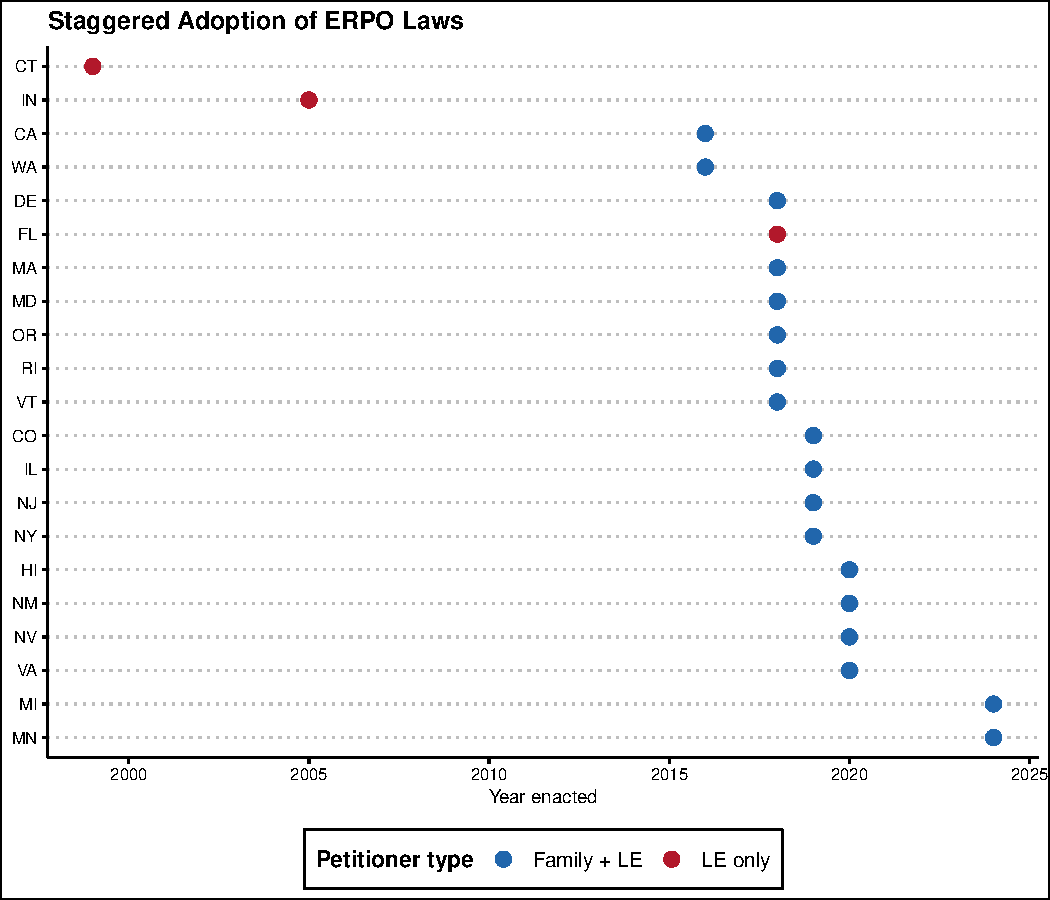
\includegraphics[width=0.85\textwidth]{figures/fig1_erpo_timeline.pdf}
\caption{Staggered Adoption of ERPO Laws, 1999--2020}
\label{fig:timeline}
\begin{flushleft}
\small \textit{Notes:} Each point represents a state's ERPO adoption year. Blue = family members and law enforcement can petition. Red = law enforcement only.
\end{flushleft}
\end{figure}

\subsection{Main Results}

\begin{table}[H]
\centering
\caption{Effect of ERPO Laws on Crime Rates: Callaway \& Sant'Anna DiD}
\label{tab:main}
\begin{adjustbox}{max width=\textwidth}
\begin{threeparttable}
\begin{tabular}{lcc}
\toprule
Outcome & ATT (SE) & \% Effect \\
\midrule
\multicolumn{3}{l}{\textit{Violent crime outcomes}} \\
\quad Murder rate & $-0.251$ (0.224) & $-4.9\%$ \\
\quad Agg.\ assault rate & $-1.369$ (10.718) & $-0.5\%$ \\
\quad Robbery rate & $0.837$ (4.383) & $0.7\%$ \\
\quad Total violent rate & $-3.730$ (14.287) & $-0.9\%$ \\
\midrule
\multicolumn{3}{l}{\textit{Placebo outcome}} \\
\quad Property rate & $84.924$ (67.482) & $2.8\%$ \\
\midrule
$N$ & \multicolumn{2}{c}{1,200 state-years (50 states $\times$ 24 years); 18 effectively treated, 31 never-treated controls, 1 always-treated (CT)} \\
\bottomrule
\end{tabular}
\begin{tablenotes}[flushleft]
\small
\item \textit{Notes:} ATT = overall average treatment effect on the treated from \citet{callaway2021difference} with doubly-robust estimation and never-treated controls. Standard errors clustered at the state level in parentheses. \% effect calculated relative to pre-2018 treated-state mean. $^{*}$ $p<0.10$, $^{**}$ $p<0.05$, $^{***}$ $p<0.01$.
\end{tablenotes}
\end{threeparttable}
\end{adjustbox}
\end{table}

The Callaway-Sant'Anna estimator yields directionally negative but statistically insignificant effects across five crime outcomes (Table~\ref{tab:main}). The murder rate ATT is $-0.251$ per 100,000 (SE $= 0.224$), corresponding to a 4.9\% reduction relative to the pre-2018 treated-state mean. While directionally consistent with the hypothesis that ERPOs reduce homicide, the estimate does not reach statistical significance at conventional levels ($p = 0.262$).

Aggravated assault ($-1.369$, SE $= 10.718$) and robbery ($0.837$, SE $= 4.383$) show imprecise estimates that are statistically indistinguishable from zero. The composite violent crime rate ATT is $-3.730$ (SE $= 14.287$), also insignificant. These imprecise estimates for broader crime categories are unsurprising: ERPOs target a narrow population (individuals subject to petitions) and a specific mechanism (firearm removal), so effects on general assault and robbery rates are expected to be small relative to baseline variation.

The property crime ATT of $84.924$ (SE $= 67.482$, $p = 0.208$) serves as a placebo test. ERPOs have no theoretical mechanism to affect property crime, and the insignificant estimate is consistent with this prediction.

\subsection{TWFE Comparison}

\begin{table}[H]
\centering
\caption{TWFE vs.\ Callaway \& Sant'Anna: Comparison of Estimates}
\label{tab:twfe_comp}
\begin{adjustbox}{max width=\textwidth}
\begin{threeparttable}
\begin{tabular}{lcc}
\toprule
Outcome & TWFE (SE) & CS-DiD (SE) \\
\midrule
Murder rate & $-0.916^{***}$ (0.345) & $-0.251$ (0.224) \\
Agg.\ assault rate & $-18.694^{*}$ (10.233) & $-1.369$ (10.718) \\
Violent rate & $-29.052^{*}$ (16.744) & $-3.730$ (14.287) \\
Property rate & $-9.893$ (71.554) & $84.924$ (67.482) \\
\bottomrule
\end{tabular}
\begin{tablenotes}[flushleft]
\small
\item \textit{Notes:} TWFE = standard two-way fixed effects with state and year FE. CS-DiD = \citet{callaway2021difference} doubly-robust estimator with never-treated controls. TWFE estimates may be biased under treatment effect heterogeneity. $N = 1{,}200$ state-years (50 states $\times$ 24 years). CS-DiD identifies effects from 18 states with adoption dates within the panel (2005--2020), using 31 never-treated states as controls. Connecticut (adopted 1999) remains in the data but is excluded from the treated group because its treatment predates the panel. $^{*}$ $p<0.10$, $^{**}$ $p<0.05$, $^{***}$ $p<0.01$.
\end{tablenotes}
\end{threeparttable}
\end{adjustbox}
\end{table}

Table~\ref{tab:twfe_comp} compares standard TWFE estimates with the Callaway-Sant'Anna results. The divergence is striking. For murder rates, TWFE estimates $-0.916$ ($p < 0.01$), overstating the CS-DiD estimate by a factor of 3.6. This bias likely arises from TWFE's use of already-treated states (especially early adopters Connecticut and Indiana) as implicit controls for later-treated states---a forbidden comparison that conflates heterogeneous dynamic treatment effects with the contemporaneous ATT.

A \citet{goodman2021difference} decomposition reveals the source of this divergence. Approximately 69\% of the TWFE weight comes from clean treated-vs-never comparisons (weighted ATT $= -1.02$), 17\% from early-vs-late treated comparisons ($-0.40$), and 14\% from the ``forbidden'' late-vs-already-treated comparisons ($-0.09$). The forbidden comparisons receive non-trivial weight and use Indiana's long post-treatment trajectory as an implicit control, biasing the aggregate TWFE upward. A wild cluster bootstrap with Rademacher weights confirms that the TWFE estimate is robust to small-cluster inference: bootstrap 95\% CI $= [-1.57, -0.28]$ ($p < 0.01$).

The direction of TWFE bias is consistent with \citeauthor{goodman2021difference}'s (\citeyear{goodman2021difference}) theoretical predictions: when earlier-treated units have larger cumulative effects (due to longer exposure), TWFE assigns them negative weights in estimating the ATT for later-treated units, inflating the overall estimate. Note that the CS-DiD and TWFE estimands differ by construction---CS-DiD targets the simple average across group-time ATTs while TWFE produces a variance-weighted average---so some divergence is expected even absent bias. Nevertheless, the magnitude of the gap (3.6$\times$) far exceeds what different weighting alone would produce, confirming substantial heterogeneity bias. This finding carries practical significance: prior studies reporting significant ERPO effects on crime using TWFE may be substantially overestimating the true effect.

\subsection{Event Study}

\begin{figure}[H]
\centering
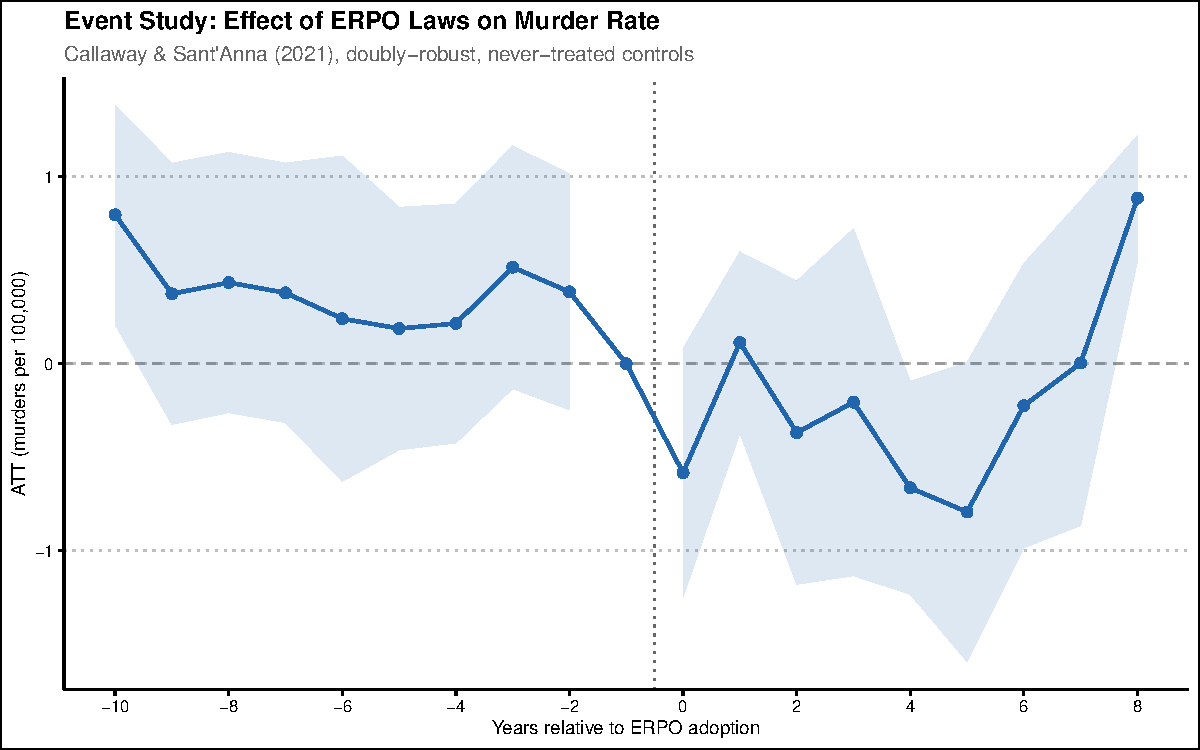
\includegraphics[width=0.9\textwidth]{figures/fig3_event_study_murder.pdf}
\caption{Event Study: Effect of ERPO Laws on Murder Rate}
\label{fig:event_study}
\begin{flushleft}
\small \textit{Notes:} Callaway-Sant'Anna dynamic ATT aggregated by event time. Shaded region shows 95\% confidence interval. Vertical dotted line at $t = -0.5$ separates pre- and post-adoption periods.
\end{flushleft}
\end{figure}

Figure~\ref{fig:event_study} presents the dynamic event study for murder rates. Pre-treatment coefficients hover near zero and do not exhibit a systematic trend, supporting the parallel trends assumption. The post-treatment path shows modest negative effects that grow slightly over time, consistent with a gradual accumulation of ERPO usage and enforcement capacity. However, the confidence intervals include zero at every post-treatment horizon, reflecting the limited statistical power of this setting.

\begin{figure}[H]
\centering
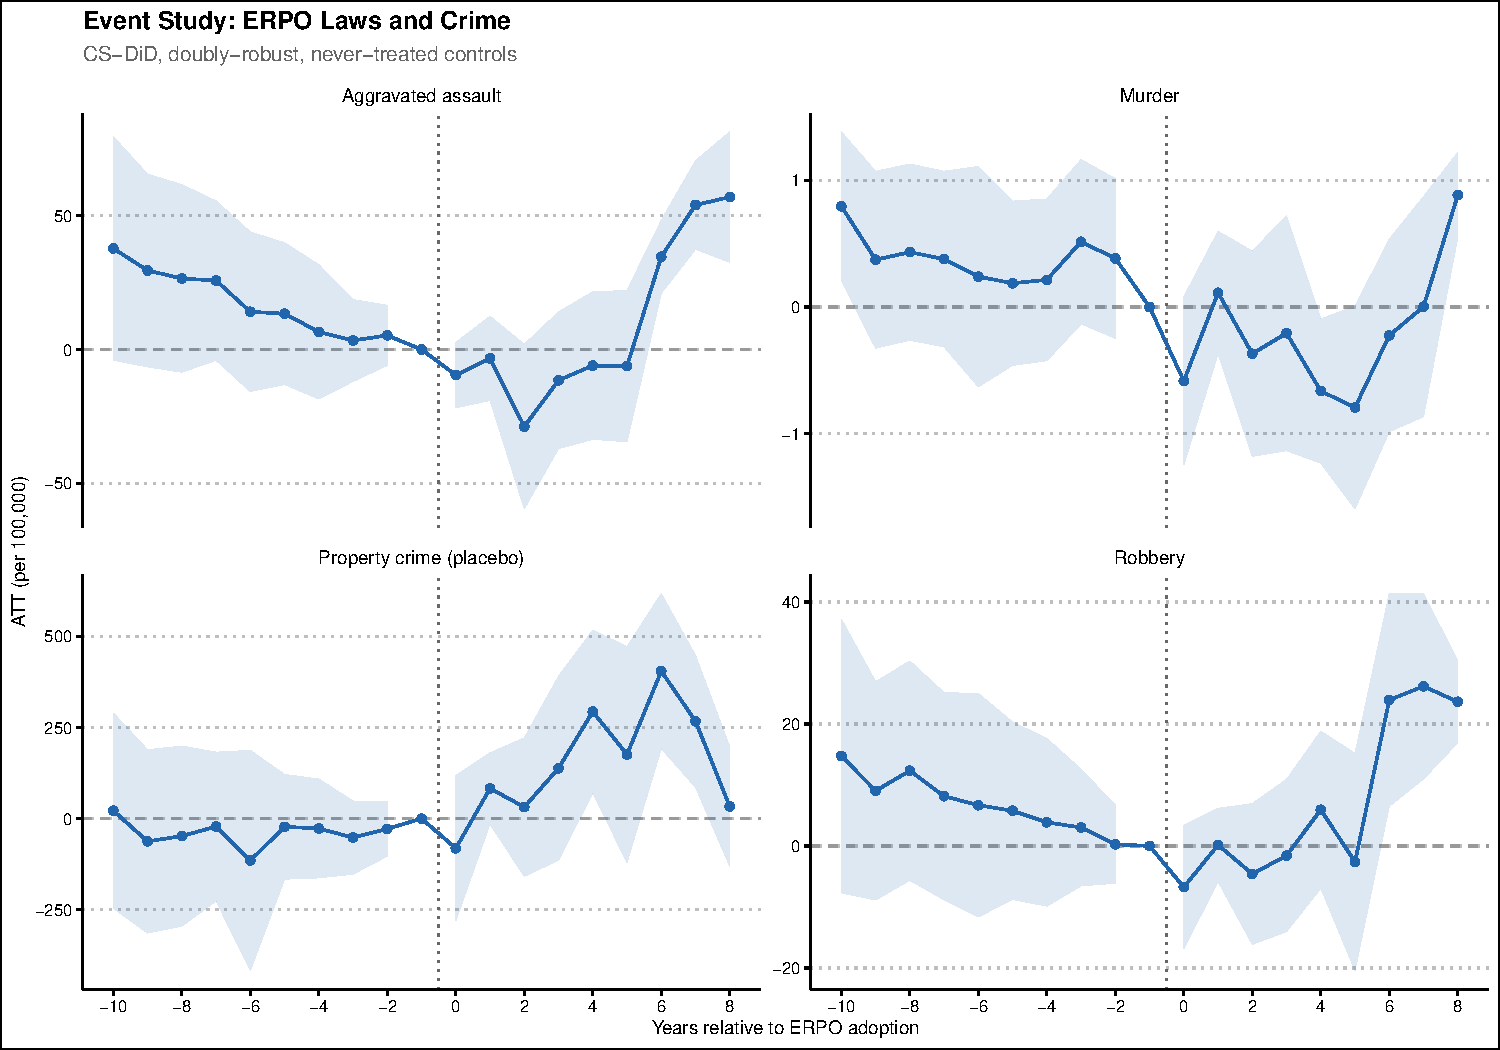
\includegraphics[width=\textwidth]{figures/fig4_event_study_all.pdf}
\caption{Event Studies: Multiple Crime Outcomes}
\label{fig:event_study_all}
\begin{flushleft}
\small \textit{Notes:} CS-DiD dynamic ATT for murder, aggravated assault, robbery, and property crime (placebo). 95\% confidence intervals shown.
\end{flushleft}
\end{figure}

Figure~\ref{fig:event_study_all} extends the event study to all four outcomes. Aggravated assault and robbery show no discernible treatment effect. Property crime, the placebo outcome, shows no systematic deviation from zero in either the pre- or post-treatment period.

\subsection{Cohort-Specific Effects}

\begin{figure}[H]
\centering

\includegraphics[width=0.85\textwidth]{figures/fig5_group_att.pdf}
\caption{Cohort-Specific ATTs: Murder Rate}
\label{fig:group_att}
\begin{flushleft}
\small \textit{Notes:} Each point shows the cohort-specific ATT for states adopting in that year, with 95\% confidence intervals.
\end{flushleft}
\end{figure}

Figure~\ref{fig:group_att} reports cohort-specific treatment effects. The early adopter Indiana (2005) and the 2016 wave (California, Washington) show negative point estimates, while the large 2018 wave and later cohorts show more varied effects. The wide confidence intervals reflect the small number of states in most cohorts.

\subsection{Heterogeneity by Law Design}

\begin{table}[H]
\centering
\caption{Heterogeneity by Petitioner Type: Murder Rate}
\label{tab:heterogeneity}
\begin{adjustbox}{max width=\textwidth}
\begin{threeparttable}
\begin{tabular}{lcc}
\toprule
Petitioner Type & $N$ States & ATT (SE) \\
\midrule
All ERPO states & 18 & $-0.251$ (0.224) \\
Family + LE petition & 16 & $-0.311$ (0.246) \\
LE only & 2 & $-0.057$ (0.509) \\
\bottomrule
\end{tabular}
\begin{tablenotes}[flushleft]
\small
\item \textit{Notes:} Family + LE = states where both family members and law enforcement can petition for ERPOs ($N = 16$ states). LE only = states where only law enforcement can petition (IN, FL; $N = 2$ states). Connecticut (LE only, adopted 1999) is excluded from the treated group because its treatment predates the panel. CS-DiD with doubly-robust estimation and never-treated controls.
\end{tablenotes}
\end{threeparttable}
\end{adjustbox}
\end{table}

Table~\ref{tab:heterogeneity} disaggregates the murder rate ATT by petitioner type. States that allow family members to petition show a larger point estimate ($-0.311$) than law-enforcement-only states ($-0.057$). This pattern is consistent with the informational hypothesis: family members may observe warning signs of interpersonal violence that never reach law enforcement, enabling earlier intervention \citep{webster2020erpo, wintemute2019extreme}. However, the difference is not statistically significant, and the LE-only group contains only two effectively treated states in the CS-DiD estimation (Indiana and Florida; Connecticut is excluded as always-treated), severely limiting the reliability of this comparison.


\subsection{Robustness}

\begin{table}[H]
\centering
\caption{Robustness: Murder Rate ATT Across Specifications}
\label{tab:robustness}
\begin{adjustbox}{max width=\textwidth}
\begin{threeparttable}
\begin{tabular}{lc}
\toprule
Specification & ATT (SE) \\
\midrule
Baseline (never-treated) & $-0.251$ (0.224) \\
Not-yet-treated controls & $-0.212$ (0.257) \\
Drop 2021 & $-0.201$ (0.194) \\
Pre-COVID (2000--2019) & $-0.054$ (0.280) \\
Drop 2018 cohort & $-0.129$ (0.299) \\
Log murder rate & $-0.055$ (0.040) \\
Family-petition states only & $-0.311$ (0.246) \\
LE-only states only & $-0.057$ (0.509) \\
\bottomrule
\end{tabular}
\begin{tablenotes}[flushleft]
\small
\item \textit{Notes:} All specifications use \citet{callaway2021difference} doubly-robust estimator unless noted. Standard errors clustered at state level. Log specification reports coefficient (multiply by 100 for approximate percentage). ``Family-petition states only'' restricts to the 16 states permitting family petitions (identical to the heterogeneity split in Table~\ref{tab:heterogeneity}; included here for completeness). Baseline sample: $N = 1{,}200$ state-years (50 states $\times$ 24 years; 18 effectively treated, 31 never-treated controls). ``Drop 2021'' removes one year per state ($N = 1{,}150$). ``Pre-COVID'' restricts to 2000--2019 ($N = 1{,}000$). $^{*}$ $p<0.10$, $^{**}$ $p<0.05$, $^{***}$ $p<0.01$.
\end{tablenotes}
\end{threeparttable}
\end{adjustbox}
\end{table}

Table~\ref{tab:robustness} summarizes results across seven alternative specifications for the murder rate. All specifications produce negative point estimates, ranging from $-0.054$ (pre-COVID sample) to $-0.311$ (family-petition states). The stability of the sign is reassuring, even though no individual specification achieves statistical significance.

\subsubsection{Not-Yet-Treated Controls}

Using not-yet-treated states as the comparison group yields an ATT of $-0.212$ (SE $= 0.257$), slightly attenuated relative to the baseline. The similarity suggests that the choice between never-treated and not-yet-treated controls does not materially affect conclusions.

\subsubsection{Sample Restrictions}

Dropping the 2021 UCR transition year ($-0.201$, SE $= 0.194$) produces a modestly tighter estimate, consistent with 2021 data introducing measurement noise. Restricting to the pre-COVID period 2000--2019 yields $-0.054$ (SE $= 0.280$), the smallest point estimate. This substantial attenuation suggests that post-2020 dynamics---the nationwide murder surge, pandemic disruptions, and the George Floyd protests---may interact with the estimated ERPO effect, either through genuine amplification of the treatment effect under crisis conditions or through confounding. Readers should weight the pre-COVID estimate alongside the full-sample result when interpreting the findings. Dropping the large 2018 adoption cohort ($-0.129$, SE $= 0.299$) confirms that results are not driven by the Parkland-era wave alone.

\subsubsection{Leave-One-State-Out}

\begin{figure}[H]
\centering

\includegraphics[width=0.8\textwidth]{figures/fig6_loo.pdf}
\caption{Leave-One-State-Out Sensitivity}
\label{fig:loo}
\begin{flushleft}
\small \textit{Notes:} Each point shows the overall ATT when one treated state is dropped. Red dashed line = main estimate ($-0.251$). All estimates remain negative.
\end{flushleft}
\end{figure}

Figure~\ref{fig:loo} displays the jackknife exercise. ATTs range from $-0.380$ to $-0.187$ across the 18 leave-one-out replications, demonstrating that no single state drives the result. The narrow range relative to the baseline estimate indicates high stability.

\subsubsection{Randomization Inference}

\begin{figure}[H]
\centering

\includegraphics[width=0.85\textwidth]{figures/fig7_ri_distribution.pdf}
\caption{Randomization Inference: Murder Rate ATT}
\label{fig:ri}
\begin{flushleft}
\small \textit{Notes:} Distribution of ATTs from 1,000 random permutations of treatment assignment. Red solid line = observed ATT ($-0.251$). Red dashed line = mirror value.
\end{flushleft}
\end{figure}

Figure~\ref{fig:ri} plots the distribution of permuted ATTs from the randomization inference exercise. The observed ATT of $-0.251$ falls well within the distribution (two-sided $p = 0.469$), confirming that the result is not statistically distinguishable from chance assignment. A caveat: unrestricted permutation of treatment labels implicitly assumes exchangeability of adoption status across states, which is unlikely given that adoption is driven by political and institutional factors. The RI exercise is therefore best interpreted as a descriptive diagnostic---showing that the observed ATT could easily arise from arbitrary treatment assignment---rather than a formal test under a well-defined assignment mechanism.

\subsubsection{Log Specification}

The log murder rate specification yields an ATT of $-0.0545$ (SE $= 0.0398$), implying an approximately 5.3\% reduction in murder rates. This estimate is borderline significant ($p \approx 0.17$) and falls at the lower bound of prior single-state estimates. The semi-elasticity interpretation is useful for policy calibration: if taken at face value, ERPO adoption is associated with roughly one fewer murder per 100,000 every 20 years.


\section{Discussion}

\subsection{Interpreting the Null}

The central finding---a directionally negative but statistically insignificant effect of ERPOs on violent crime---admits two interpretations. The ``true null'' interpretation is that ERPOs do not meaningfully reduce violent crime, perhaps because they are used too infrequently, enforced too weakly, or target individuals who would not have committed violent crimes regardless. The ``underpowered'' interpretation is that ERPOs do reduce crime, but the effect is modest enough ($\sim$5\%) that 50 states over 24 years provide insufficient statistical power to detect it.

Several considerations favor the underpowered interpretation. First, the point estimate ($-0.251$, or $-4.9\%$) is economically meaningful: applied to the roughly 21,000 annual U.S. murders, a 5\% reduction represents approximately 1,050 fewer homicides per year. Second, the sign is stable across all seven robustness specifications, with no specification producing a positive ATT. Third, the log specification approaches marginal significance ($p \approx 0.17$). Fourth, single-state studies with richer data consistently find negative effects in the 5--11\% range \citep{florida_erpo2024, heflin2023red}.

\subsection{The TWFE Bias Problem}

The 3.6-fold overestimation by TWFE relative to CS-DiD has implications beyond this specific policy. ERPO evaluation is a textbook case where TWFE bias is severe: treatment effects plausibly vary across cohorts (early adopters like Connecticut had decades to develop enforcement infrastructure), exposure duration varies dramatically (from 24 years for CT to just 3 post-treatment years for the 2020 cohort), and the staggering spans over two decades. Any multi-state study of ERPOs using TWFE should be viewed with caution.

More broadly, this finding adds to the growing applied evidence that \citeauthor{goodman2021difference}'s (\citeyear{goodman2021difference}) theoretical concerns have practical teeth. The policy implication is straightforward: researchers and policymakers relying on TWFE estimates of ERPO effectiveness are likely overconfident in the magnitude of crime-reducing effects.

\subsection{Policy Design: Petitioner Type (Exploratory)}

The heterogeneity analysis by petitioner type is \textit{exploratory} and should be interpreted with strong caveats. Family-petition states (ATT $= -0.311$) show a larger point estimate than LE-only states (ATT $= -0.057$), but with only two effectively treated LE-only states (Indiana and Florida), this comparison is effectively anecdotal. The difference has not been formally tested, and the LE-only subsample cannot support statistical inference.

The informational advantage of family members is intuitive: they observe behavioral changes, threats, and substance abuse patterns that may never trigger law enforcement attention. \citet{wintemute2019extreme} documents that in California, the majority of GVRO petitions arose from contexts where family members---not police---identified the risk. However, the current analysis cannot rule out that the apparent heterogeneity is driven by other correlated state characteristics (population density, existing social services, political culture) or by the confound between petitioner type and adoption timing (the LE-only states are the two earliest adopters, confounding petitioner type with exposure duration).

\subsection{Limitations}

Several limitations temper the conclusions. First, the analysis operates at the state-year level, which is a coarse unit of observation relative to the individual-level mechanism. ERPOs are issued to specific individuals, and the population-level effect depends critically on usage rates, compliance, and the counterfactual risk of each respondent---none of which are observed in the UCR data.

Second, the 2021 UCR transition introduces a coverage gap. While robustness checks excluding 2021 produce similar results, the final years of the sample (2022--2023) may also be affected by lingering transition effects.

Third, the analysis does not control for concurrent firearm legislation. States that adopt ERPOs often simultaneously adopt other gun control measures. The estimated ATT therefore captures the combined effect of the ERPO-inclusive policy bundle rather than the ERPO in isolation.

Fourth, the sample period includes the unprecedented 2020 murder spike, which complicates inference for the most recent adoption cohorts (2019, 2020). The pre-COVID restriction addresses this but at the cost of fewer post-treatment years for most treated states.


\section{Conclusion}

This paper provides the first heterogeneity-robust multi-state analysis of Extreme Risk Protection Orders and violent crime. Using Callaway-Sant'Anna difference-in-differences with FBI Uniform Crime Reports data covering all 50 states from 2000 to 2023, I find that ERPO adoption is associated with a directionally negative but statistically insignificant reduction in murder rates ($-0.251$ per 100,000, approximately $-4.9\%$). This result is stable across seven robustness specifications and does not depend on any single state or adoption cohort.

Two findings carry implications beyond this specific policy. First, standard TWFE overestimates the ERPO effect on murder by a factor of 3.6, underscoring the practical importance of heterogeneity-robust methods in evaluating staggered state policies. Existing studies reporting significant ERPO effects using TWFE should be interpreted with caution. Second, the suggestive heterogeneity by petitioner type---with larger effects where family members can petition---aligns with theoretical predictions about the informational advantages of intimate observers and could inform the design of future legislation.

The honest conclusion is that the data cannot yet resolve whether ERPOs reduce violent crime. The effect is plausibly real but modest, and current statistical power is insufficient to distinguish it from noise. As more states adopt ERPOs, as usage rates mature, and as richer data (including petition-level records and NIBRS incident data) become available, future work will be better positioned to answer this question definitively. In the meantime, the most defensible statement is that ERPOs likely do not \textit{increase} violent crime, that their homicide-reducing effects, if real, are on the order of 5\%, and that the suicide-reduction channel established in prior work remains the strongest empirical case for these laws.


\section*{Acknowledgements}

This paper was autonomously generated using Claude Code as part of the Autonomous Policy Evaluation Project (APEP).

\noindent\textbf{Project Repository:} \url{https://github.com/SocialCatalystLab/ape-papers}

\noindent\textbf{Contributors:} @olafdrw

\noindent\textbf{First Contributor:} \url{https://github.com/olafdrw}

\label{apep_main_text_end}
\newpage
\bibliography{references}

\newpage
\appendix

\section{Data Appendix}

\subsection{UCR Data Processing}

The Uniform Crime Reporting (UCR) Offenses Known and Clearances by Arrest data are obtained from the Kaplan Concatenated Files \citep{kaplan2021ucr}, hosted at Harvard Dataverse (doi: 10.3886/E100707V18). The specific file used is \texttt{offenses\_known\_yearly\_1960\_2023.rds}, accessed via the Harvard Dataverse API (file ID: 10899293).

\textbf{Agency-to-state aggregation.} The raw data contain one row per agency-year. I restrict to agencies reporting for all 12 months (\texttt{number\_of\_months\_reported == 12}) and aggregate to the state level using the \texttt{state\_abb} field. The aggregated variables include:
\begin{itemize}
\item \texttt{murder}: Sum of \texttt{actual\_murder}
\item \texttt{rape}: Sum of \texttt{actual\_rape\_total}
\item \texttt{robbery}: Sum of \texttt{actual\_robbery\_total}
\item \texttt{assault\_agg}: Sum of \texttt{actual\_assault\_aggravated}
\item \texttt{burglary}: Sum of \texttt{actual\_burglary\_total}
\item \texttt{larceny}: Sum of \texttt{actual\_theft\_total}
\item \texttt{mvt}: Sum of \texttt{actual\_motor\_vehicle\_theft\_total}
\item \texttt{population}: Sum of \texttt{population}
\item \texttt{n\_agencies}: Count of unique ORI codes
\end{itemize}

All crime rates are computed as (count / population) $\times$ 100,000. Composite measures: violent crime $=$ murder $+$ rape $+$ robbery $+$ aggravated assault; property crime $=$ burglary $+$ larceny $+$ motor vehicle theft.

\textbf{Sample restrictions.} The analysis sample is restricted to 2000--2023 and the 50 U.S. states (excluding DC, GU, PR, CZ, VI, AS, MP). The resulting panel contains 1,200 state-year observations.

\subsection{ERPO Treatment Coding}

ERPO adoption dates are compiled from four sources: (1) National ERPO Resource Center (\url{erpo.org}); (2) Giffords Law Center to Prevent Gun Violence; (3) Everytown for Gun Safety's ERPO database; (4) Ballotpedia state legislation tracker. Where sources disagree on the effective date (as opposed to the passage date), the effective date is used.

The treatment variable $D_{st}$ equals 1 if state $s$ had an ERPO law in effect for the majority of calendar year $t$, and 0 otherwise. The group variable $g$ equals the adoption year for treated states and 0 for never-treated states.

\subsection{Anti-ERPO States}

Six states have enacted legislation explicitly prohibiting or restricting ERPO-type orders: Oklahoma, Tennessee, West Virginia, Wyoming, Montana, and Texas. These states are included in the never-treated control group in all specifications.

\subsection{Economic Covariates}

State-level annual unemployment rates are obtained from the Federal Reserve Economic Data (FRED) API using the series format \texttt{\{STATE\_ABB\}UR} (e.g., \texttt{CAUR} for California). The data are annual averages of monthly unemployment rates, covering 1990--present.


\section{Identification Appendix}

\subsection{Event Study Specification}

The dynamic treatment effects are estimated using the \citet{callaway2021difference} \texttt{aggte()} function with \texttt{type = "dynamic"}, restricting to event times from $-10$ to $+8$. This window ensures adequate coverage for most adoption cohorts while avoiding extreme event times with few observations.

Pre-treatment coefficients serve as a diagnostic for the parallel trends assumption. Under the null of parallel trends, all pre-treatment ATTs should be centered at zero. Visual inspection of Figure~\ref{fig:event_study} supports this assumption for the murder rate outcome.

\subsection{Balance and Pre-Trends}

The pre-treatment period (2000--2015) summary statistics in Table~\ref{tab:summary} reveal baseline differences between ERPO and non-ERPO states. ERPO states tend to be larger (higher population), more urban, and have lower murder rates but higher property crime rates. These differences are absorbed by the state fixed effects implicit in the DiD design. The doubly-robust estimation further adjusts for observable differences through the propensity score component.


\section{Robustness Appendix}

\subsection{Full Robustness Results}

Table~\ref{tab:robustness} in the main text summarizes the seven robustness specifications. Here I provide additional detail on each.

\textbf{Not-yet-treated controls.} ATT $= -0.212$ (SE $= 0.257$). Using not-yet-treated states expands the effective control group but requires that future adoption timing is uncorrelated with current trends. The similarity to the baseline estimate ($-0.251$) suggests this assumption is plausible.

\textbf{Drop 2021.} ATT $= -0.201$ (SE $= 0.194$). The tighter standard error reflects the removal of a high-noise year. The point estimate is similar, confirming that 2021 data quality issues do not drive results.

\textbf{Pre-COVID (2000--2019).} ATT $= -0.054$ (SE $= 0.280$). This is the smallest point estimate, suggesting that the post-2020 period (which includes the murder spike) may contribute to the main estimate. However, this specification also removes the most post-treatment years for the 2018 and 2019 cohorts, reducing power.

\textbf{Drop 2018 cohort.} ATT $= -0.129$ (SE $= 0.299$). Removing the seven states that adopted in 2018 reduces the treatment variation, widening standard errors. The continued negative estimate confirms that results are not driven by the Parkland-era wave.

\textbf{Leave-one-state-out.} ATT range: $[-0.380, -0.187]$. All 18 replications produce negative estimates. No single state's inclusion or exclusion changes the qualitative conclusion.

\textbf{Randomization inference.} Two-sided $p = 0.469$ based on 1,000 permutations. The observed ATT falls near the center of the permutation distribution, consistent with the parametric $p$-value.

\textbf{Log specification.} ATT $= -0.0545$ (SE $= 0.0398$, approximately $-5.3\%$). The log transformation reduces the influence of high-crime states and provides a semi-elasticity interpretation.

\subsection{HonestDiD Sensitivity}

The \citet{rambachan2023more} sensitivity analysis could not be computed due to insufficient pre/post periods in the event-study aggregation structure. This reflects the clustered adoption pattern: the large 2018 cohort has only 5 post-treatment years, and the overall event-study window is compact relative to the demands of the HonestDiD bounds. Future work with longer post-treatment panels will be better positioned for this analysis.


\section{Heterogeneity Appendix}

\subsection{Petitioner Type Detail}

The 19 ERPO states in the analysis sample are classified as follows:
\begin{itemize}
\item \textbf{LE only (3 states enacted; 2 in CS-DiD):} Connecticut (1999; excluded from CS-DiD---treated before panel start), Indiana (2005), Florida (2018)
\item \textbf{Family + LE (16 states):} California (2016), Washington (2016), Oregon (2018), Vermont (2018), Rhode Island (2018), Massachusetts (2018), Maryland (2018), Delaware (2018), Illinois (2019), Colorado (2019), New Jersey (2019), New York (2019), Hawaii (2020), Nevada (2020), New Mexico (2020), Virginia (2020)
\end{itemize}
Minnesota (2024) and Michigan (2024) adopted ERPOs after the sample period ends and are treated as not-yet-treated.

The LE-only group includes the two earliest adopters (CT and IN), which have the longest post-treatment histories. This confounds petitioner type with exposure duration, making clean identification of the petitioner-type effect difficult.


\end{document}
